\documentclass[twoside]{article}


\usepackage[sc]{mathpazo} % Use the Palatino font
\usepackage[T1]{fontenc} % Use 8-bit encoding that has 256 glyphs
\linespread{1.05} % Line spacing - Palatino needs more space between lines
\usepackage{microtype} % Slightly tweak font spacing for aesthetics

\usepackage[hmarginratio=1:1,top=32mm,columnsep=20pt]{geometry} % Document margins
\usepackage{multicol} % Used for the two-column layout of the document
\usepackage[hang, small,labelfont=bf,up,textfont=it,up]{caption} % Custom captions under/above floats in tables or figures
\usepackage{booktabs} % Horizontal rules in tables
\usepackage{float} % Required for tables and figures in the multi-column environment - they need to be placed in specific locations with the [H] (e.g. \begin{table}[H])
\usepackage{hyperref} % For hyperlinks in the PDF

\usepackage{lettrine} % The lettrine is the first enlarged letter at the beginning of the text
\usepackage{paralist} % Used for the compactitem environment which makes bullet points with less space between them

\usepackage{titlesec} % Allows customization of titles
\renewcommand\thesection{\Roman{section}} % Roman numerals for the sections
\renewcommand\thesubsection{\Roman{subsection}} % Roman numerals for subsections
\titleformat{\section}[block]{\large\scshape\centering}{\thesection.}{1em}{} % Change the look of the section titles
\titleformat{\subsection}[block]{\large}{\thesubsection.}{1em}{} % Change the look of the section titles

\usepackage{fancyhdr} % Headers and footers
\pagestyle{fancy} % All pages have headers and footers
\fancyhead{} % Blank out the default header
\fancyfoot{} % Blank out the default footer
\fancyhead[C]{USC EE511-PROJECT2} % Custom header text
\fancyfoot[RO,LE]{\thepage} % Custom footer text



\usepackage{multicol}
\usepackage{listings}
\usepackage{graphicx}
\usepackage{caption}
\usepackage{subcaption}
\usepackage{hyperref}
\usepackage{color}
\usepackage{float}
\usepackage{mathtools}
\usepackage{amssymb}
\usepackage{wrapfig}

%----------------------------------------------------------------------------------------
%	TITLE SECTION
%----------------------------------------------------------------------------------------

\title{\vspace{-15mm}\fontsize{24pt}{10pt}\selectfont\textbf{Project \#2 - Samples and Statistics }} % Article title

\author{
\large
\textsc{Li Yicheng}\thanks{\href{https://github.com/IAMLYCHEE/EE511-PROJECT3}{github link: https://github.com/IAMLYCHEE/EE511-PROJECT1} }\\[2mm] % Your name
\normalsize USCID:7827077047\\
\normalsize email: l.y.c.liyicheng@gmail.com \\ % Your institution
\normalsize USC Viterbi of Engineering
\vspace{-5mm}
}

\lstset{ %
language=Matlab,                % choose the language of the code
basicstyle=\footnotesize,       % the size of the fonts that are used for the code
numbers=left,                   % where to put the line-numbers
numberstyle=\footnotesize,      % the size of the fonts that are used for the line-numbers
stepnumber=1,                   % the step between two line-numbers. If it is 1 each line will be numbered
numbersep=5pt,                  % how far the line-numbers are from the code
backgroundcolor=\color{white},  % choose the background color. You must add \usepackage{color}
showspaces=false,               % show spaces adding particular underscores
showstringspaces=false,         % underline spaces within strings
showtabs=false,                 % show tabs within strings adding particular underscores
frame=single,           % adds a frame around the code
tabsize=2,          % sets default tabsize to 2 spaces
captionpos=b,           % sets the caption-position to bottom
breaklines=true,        % sets automatic line breaking
breakatwhitespace=false,    % sets if automatic breaks should only happen at whitespace
escapeinside={\%*}{*)}          % if you want to add a comment within your code
}

\date{}

%----------------------------------------------------------------------------------------

\begin{document}

\maketitle % Insert title

\thispagestyle{fancy} % All pages have headers and footers
\section{microchips test}
\subsection{\normalsize{Problem Description}}
(a) There is a batch of 125 microchips, if the distributor find any defective microchip in the chosen microchip, the batch of microchips would be rejected. Suppose there are 6 defective units in the lot, what is the probabilty that the distributor will reject the lot if five microchips are tested.\\
(b) What is the fewest number of microchips that the distributor should test to reject this lot 95\% of the time.\\
\subsection {\normalsize{Experiment(a)}}
A function called reject\_prop is generated to show the probability that the distributor would reject the lot with test\_amount microchips were tested.\\[10pt]
\underline{\emph{Algorithm:}} \\[10pt]
*1.Let the defective microchip be No.1 to No.6.\\
*2.Generate test\_amount samples uniformly in 1 to 125\\
*3.If there exist index form 1 to 6, reject times plus one\\
*4.Repeat the above routine 20000 times, calculate the amount of rejections in the 20000 times, to derive the rejection probability\\

\subsection{\normalsize{core code: filename: reject\_prop.m}}
\begin{lstlisting}
function reject_p = reject_prop(test_amount)
%usage: reject_p = reject_prop(test_amount)
%given the test amount, output the reject probability
% input : test_amount : the test amount
% output: reject_p: reject probability
reject = 0;
for i = 1 : 20000 %to be accurate enough, do 20000 trial
    samples = randperm(125,test_amount);%select test amount microchips 
    if ( sum(samples < 7) > 0) %let defective chips be No.1 to No.6 , if any of these number is tested just reject
        reject = reject +1; %reject,detected such defective chip
    end
end
reject_p = reject / 20000;
\end{lstlisting}

\subsection{\normalsize{Result(a) \& Analysis:}}
If 5 chips were tested, we query:
reject\_p = reject\_prop(5)\\
\emph{we get:}\\
reject\_p = 0.2181 \\
This means, in this simulation, if 5 microchips were tested, the distributor has a probability near 22\% to reject the lot.\\
Let us compare this to the theoretical value. Because the probabilty that the distributor does not reject the lot is easier to compute, we compute that number. Using combination knowledge, we choose 5 from 199 good chips and we choose 5 from all microchips.\\
$\mathbb{P}(not \ reject) = \frac{\binom {119}{5}}{\binom {125}{5}}=0.7787\\
\mathbb{P}(reject) = 1 - \mathbb{P}(not \ reject)=0.2213\\$
Compare to our result 0.2181, they are very close.\\

\subsection{\normalsize{Experiment(b)}}
We make use of the function generated in experiment(a), we just need to change the input parameter, let it increase, until the probabilty reach 95\%, then we record the test\_amount.\\[10pt]
\emph{Algorithm:}\\[10pt]
*1.Calculate the reject probabilty under test\_amount\\
*2.If the probability is less than 95\%, increase the test\_amount\\
*3.else record the test\_amount\\
\subsection{\normalsize{core code:  filename: solution1.m}}
\begin{lstlisting}
test_amount = 5;
while(1)
    p = reject_prop(test_amount);
    if p < 0.95
        test_amount = test_amount + 1;
    else
        break
    end
end
\end{lstlisting}
\subsection{\normalsize{Result(b) \& Analysis}}
It is not a function file, just run it.\\
\emph{we get:}
test\_amount = 49\\
that means, if the distributor test 49 microchips, there is a probability of 95\% that he would reject the lot.\\
Also, let us to compare this to our theoretical value, this time the equation should be:\\
$\mathbb{P}(reject)= 1- \frac{\binom{119}{x}}{\binom{125}{x}}= 0.95\\[10pt]$
Actually, in matlab, if you compute like $\binom{119}{59}$, it may not give accurate answer,(the number is too large!), so we simplfy the formular.\\
$\frac{\binom{119}{x}}{\binom{125}{x}}= \frac{ \frac{119!}{(119-x)!x!} }{ \frac{125!}{(125-x)!x!} } = \frac{119!(125-x)!}{125!(119-x)!} =\frac{(125-x)(124-x)(123-x)(122-x)(121-x)(120-x)}{125\cdot124\cdot123\cdot122\cdot121\cdot120}=\frac{\binom{125-x}{6}}{\binom{125}{6}}\\[15pt] $
$x = 50, \mathbb{P}(reject)=0.9571\\
x = 49, \mathbb{P}(reject)=0.9534\\
x = 48, \mathbb{P}(reject)=0.9495\\
x = 47, \mathbb{P}(reject)=0.9452\\$
Therefore, the theoretical value fit our experiment result.\\
If the distributor would like to reject the lot 95\% of the time, he should take 48 or 49 chips to test.\\

\section{number of events in specified intervals} 
\subsection{\normalsize{Probelm Description}}
(a)Suppose 120 cars arrive at a freeway onramp per hour on average, simulate one hour of arrivals to the freeway ramp.Perform a Bernoulli trial to indicate a car arrival within small time interval.\\
(b)Sampling directly form an equivalent Possion distribution by using inverse transform method.Generate a histogram for the number of arrivals using this method.\\



\subsection{\normalsize{Experiment(a)}}
The requirement is to derive the amount of cars at some position per hour,suppose we divide one hour into 5000 intervals, the probabilty of one car is within this interval is $\mathbb{P}(within \ the \ interval)=\frac{120}{5000}$ and we count whether there is a car in one interval by generating a random number form the u(0,1) distribution.\\[10pt]
\underline{\emph{Algorithm}}\\[10pt]
*1.Generate N random variables from uniform distribution [0,1], N is the number of time interval.\\
*2.Count the number of these variable whose value is smaller than 120/N. Record the sum as one trial result.\\
*3.Repeat 1,2 to get more trial results and generate the histogram.\\
\subsection{\normalsize{Core Code: filename: solution2.m (part of code)}}
\begin{lstlisting}
function solution2(trial_budget,lambda)
%usage: compute the B-trial result, inverse sampling method, and theoretical value,fora possion distribution event
%input: trial times, the expected average of occurence of event (lambda)

%----------------------------------------------------------------
%theoretical p.m.f of Possion distribution
P_the = zeros(1,lambda*1.5); %record the P theoretical value
x = 1 : lambda*1.5;
for k = 1 : lambda*1.5  
    P_the(k) = trial_budget*lambda^k * exp(-lambda)/factorial(k);
end
%----------------------------------------------------------------
%Bernoulli trial method
success_amount = zeros(trial_budget,1);
N = 5000;
P = lambda / N;
for i = 1: trial_budget
    success_amount(i) = sum(rand(N,1) < P);
end
subplot(1,2,1)
histogram(success_amount,lambda*1.5,'BinLimits',[1,lambda*1.5]);
title('Bernoulli trial')
xlabel('number of cars')
ylabel('appear times')
%set the same x-axis [1,lambda*1.5] for comparing
hold on
plot(x,P_the,'r--o');
hold off
legend('B-trial','theoretical');
\end{lstlisting}



\subsection{\normalsize{Experiment(b)}}
The inverse tranform method.Inverse transformation sampling takes uniform samples of a number ${\displaystyle u}$ u between 0 and 1, interpreted as a probability, and then returns the largest number ${\displaystyle x}$ x from the domain of the distribution ${\displaystyle P(X)}$ such that ${\displaystyle P(-\infty <X<x)\leq u}$. For example, possion has a distribution of $\mathbb{P}(X = i)=\frac{e^{-\lambda}\lambda^i}{i!}$, we know that $\displaystyle\sum_{i=1}^{\infty}\mathbb{P}(X=i)=1$,first generate a random varible u from uniform distribution [0,1], and then we just accumulate $\mathbb{P}$ from $\mathbb{P}(X = 1)$ until $\displaystyle\sum_{1}^{N}\mathbb{P}(X = i)$reach u, record the N.\\[10pt]
\underline{\emph{Algorithm:}}\\[10pt]
*1.Generate a standard uniform distribution variable u, initiate P and accumulate sum F to be P(X=1).\\
*2.If u > F, F + $P_{next}$ , else break, record the accumulated index i.\\
*3.Generate i within trial budget. \\
\emph{the above generate one sample using inverse sampling method}\\
\subsection {\normalsize{Core Code :}}
\noindent \textbf {file: gen\_one\_possion.m}
\begin{lstlisting}
function i = gen_one_possion(lambda)
%usage function x = gen_one_possion(lambda)
u = rand(1);
i = 0;
p = exp(-lambda);
F = p;
while u > F
    p = lambda * p / (i+1);
    F = F + p; %accumulate
    i = i+1;
end
\end{lstlisting}
\noindent \textbf {file: solution2.m (inverse sample part)}
\begin{lstlisting}
%---------------------------------------------------
%inverse tranform method
amount_gened = zeros(trial_budget,1); %generated amount
for i = 1: trial_budget
    amount_gened(i) = gen_one_possion(lambda);
end
subplot(1,2,2)
histogram(amount_gened,lambda*1.5,'BinLimits',[1,lambda*1.5]);
title('inverse-transform method');
xlabel('number of cars')
ylabel('appear times')
hold on 
plot(x,P_the,'r--o');
hold off
legend('inverse-sample','theretical');
\end{lstlisting}
\subsection{\normalsize{Result (a),(b) \& Analysis}}
\noindent \textbf {query: solution2(10000,120)}
\begin{figure}[H]%  figure placement: here, top, bottom, or page
   \centering
   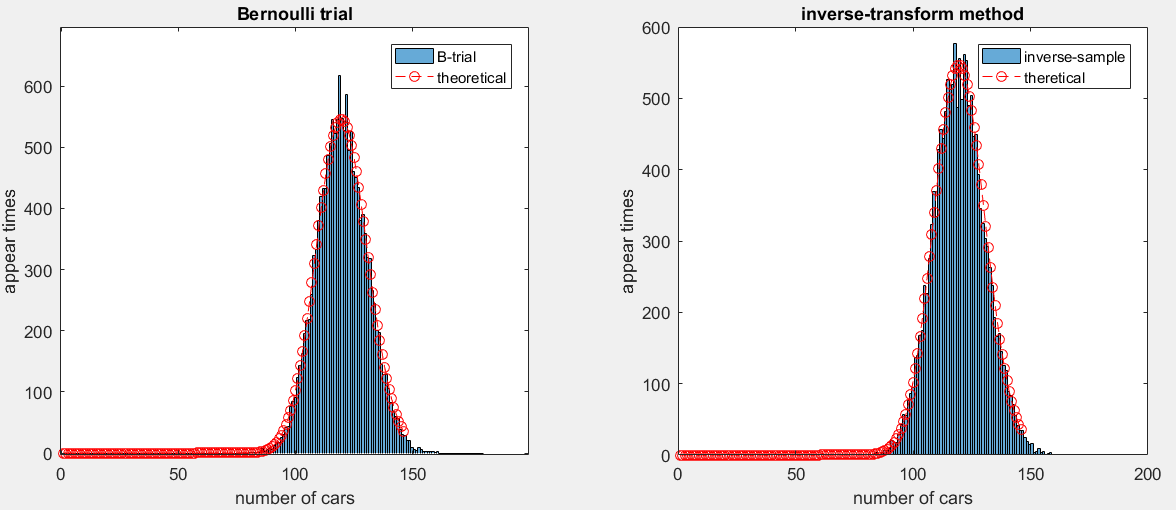
\includegraphics[width = 0.95\textwidth]{../data/solution2.png}  
   \caption{outcome histogram}
\end{figure}
\noindent From the figure, it is easy to observe that both the Bernoulli trial and the inverse sampling method reached the theoretical outcome. Both all even had more probability to get 120 cars. \\
For Bernoulli trial, theoretically, \\
$\binom{n}{k}p^k(1-p)^{n-k} \rightarrow e^{-r}\frac{r^k}{k!} $ when $n \rightarrow \infty$\\
In these case, the n is 5000, and the p is 12/5000, nearly zero. So the above convergence is suitable in this case.\\
For the inverse sampling method.\\
Let $F$ be a continuous cumulative distribution function, and let $F^{-1}$ be its inverse function.\\
$\displaystyle F^{-1}(u)=\inf \;\{x\mid F(x)\geq u\}\qquad (0<u<1).$ \\
Proof:\\
${\displaystyle {\begin{aligned}&\Pr(F^{-1}(U)\leq x)\\&{}=\Pr(U\leq F(x))\quad &({\text{applying }}F,{\text{ to both sides}})\\&{}=F(x)\quad &({\text{because }}\Pr(U\leq y)=y)\end{aligned}}}$ \\
\emph{reference:https://en.wikipedia.org/wiki/Inverse\_transform\_sampling}\\
Therefore the inverse sampling method is good for generating sample numbers at random from any probability distribution given its cumulative distribution function.\\

\section{amount of s.t.d uniform sample needed to reach sum of 4}
\subsection{\normalsize{Problem Description}}
\noindent \textbf {(a):} Generate a  random variable as the smallest number of uniform random samples whose sum is greater than four.\\
\noindent \textbf {(b):} Generate a histogram using 100,1000, and 10000 samples for N.
\subsection{\normalsize{Experiment}}
To generate random variable N is straigtforward:\\[10pt]
\underline{Algorithm:}\\[10pt]
*1:Initiate a zero sum.\\
*2:Generate a random number from standard uniform distribution. \\
*3:Add the number to the sum. loop time increase 1\\
*4: if the sum is larger than four, record the loop times and break,\\
    else goto 2.\\[10pt]
\noindent \textbf {filename: generateN.m}\\
\begin{lstlisting}
function N = generateN(thre)
%usage N = generateN(thre)
%input : thre : the threshold for sum, in this experiment , it is 4
%output: the smallest number of sum (u. random samples) > 4
sum = 0;
N = 0;
while sum < thre
    sum = sum + rand(1);
    N = N+1;
end
\end{lstlisting}
To generate histogram with defined number of N samples: and derive the expectation, just repeat the above function specific times.Use the following function to generate one histogram with specific amount of N.\\[10pt]
\noindent \textbf {filename: Nhistogram.m}\\
\begin{lstlisting}
function E = Nhistogram(eval_budget,thre)
%use: E = Nhistogram(eval_budget,thre)
% plot the histogram using eval_budget for N, threshold thre
result = zeros(eval_budget,1);
for i = 1 : eval_budget
    result(i)= generateN(thre);
end
histogram(result);
xlabel('number of uniform samples')
ylabel('appear times')
E = mean(result);
\end{lstlisting}
To get the result just use the following querys:\\
\begin{lstlisting}
subplot(1,3,1)
E_100=Nhistogram(100,4);
title('100')
subplot(1,3,2)
E_1000=Nhistogram(1000,4);
title('1000')
subplot(1,3,3)
E_10000=Nhistogram(10000,4);
title('10000')
\end{lstlisting}

\subsection{\normalsize{Result(a)(b) \& Analysis}}
\noindent \textbf {Graph:}
\begin{figure}[H]%  figure placement: here, top, bottom, or page
   \centering
   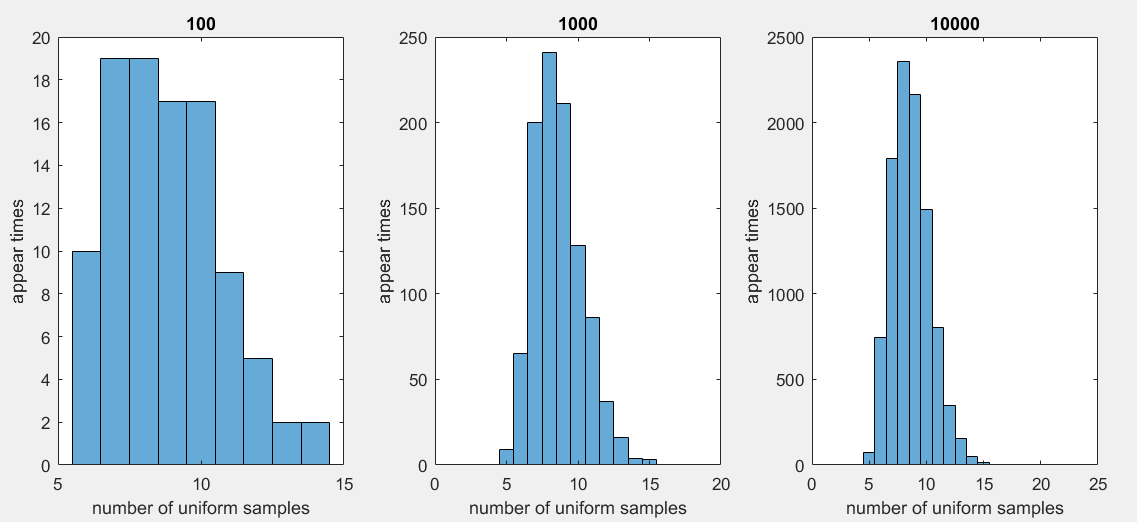
\includegraphics[width = 0.95\textwidth]{../data/solution3.png}  
   \caption{Histograms for 100,1000,10000 N samples}
\end{figure}
\noindent \textbf {Expectations}\\
E\_100 = 8.750,  E\_1000 = 8.6570, E\_10000 = 8.6652\\
\noindent \textbf {Analysis}\\
When it comes to a larger number of N, there tends to exist a convergence in the figure because it is obviously that the 1000 graph and the 10000 graph looks similar. So let us we analyse theoretical why the shape is look like this.\\
Actually, it is really difficult to generate a curve which can be described in a continous function to fit the histogram, because it only has ten more bars and it is really a discrete distribution. My thought to analyse the problem is as follows:\\
*1. Assume N numbers from standard uniform distribution have the sum larger than 4\\
*2. So k numbers is less then 4/N, while others larger than 4/N, but their average is larger than 4/N(else we can not get sum larger than 4).\\
*3. Therefore, the probabilty for N amount uniform numbers sum larger than 4 is $\mathbb{P}(N)= \binom{N}{k}(\frac{4}{N})^k(1-\frac{4}{N})^{N-k}$\\
*4. Assume k = N/2, that is half of these number is larger than 4/N, another half is smaller than 4/N\\ 
*Take a look at this distribution:  $\mathbb{P}(N)= \binom{N}{N/2}(\frac{4}{N})^{N/2}(1-\frac{4}{N})^{N-N/2}$\\
\begin{multicols}{2}
\noindent The following code are generated to analyse the above distribution function:\\
\noindent \textbf {filename: P\_n.m}\\
\begin{lstlisting}
function p = P_n(N)
p = nchoosek(N,floor(N/2))*(4/N)^(N/2)*(1-4/N)^(N-(N/2));
end
\end{lstlisting}
\noindent \textbf {filename: analysis3.m}
\begin{lstlisting}
p = zeros(1,20);
for n = 5: 17
    p(n) = P_n(n);
end
stem(p)
title('analysis')
xlabel('N')
ylabel('probability')
\end{lstlisting}
\noindent \textbf {Theoretical graph}
\begin{figure}[H]
   \centering
   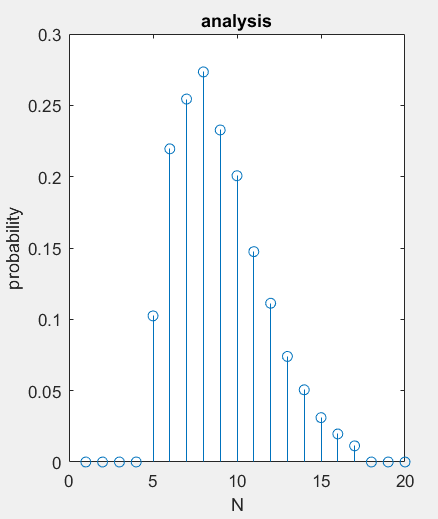
\includegraphics[width = 0.42\textwidth]{../data/analysis3.png}  
   \caption{Theoretical analysis}
\end{figure}
\end{multicols}
See, the simulation in figure 2 looks like this kind of distribution, the right side of this distribution is actually binomial distribution. Because from the formular, it is easy to derive it has the same decreasing velocity as the right side of binomial distribution.\\

\section{Some kind of sequence analysis}
\subsection{\normalsize{Problem Description}}
\noindent \textbf {(a):} we have a sequence $X_k$ where $p_j = \frac{p}{j}$ for $j = 1,2,3,\cdots 60$.Generate a historam showing the behaviour of this sequence. \\
\noindent \textbf {(b):}Define the random variable $N_j = min\{k:X_k = j\}$.Simulate sampling from $N_60$.\\

\subsection{\normalsize{Experiment(a):}}
This is like the inverse sampling method. First, [0,1] is devide into 60 parts with length $p/60,p/59,\cdots,p$ seperately. Then we generate a vairable from standard uniform distribution. And then find out what region does this varible locate.It is easier to be understand by the following algorithm.\\[10pt]
\underline{\emph{Algorithm:}}\\[10pt]
*1.Normalize p, let $\displaystyle\sum_{1}^{60}p_j=1$\\
*2.Generate a number u from standard uniform distribution\\
*3.Set accumulate number acc = p/X, X= 60\\
*4.if u > acc , stop, record X, \\
  else X = X-1,acc=acc+p/X; \\
  goto 4 again.\\
\noindent \textbf {filename: generateX.m}\\
\begin{lstlisting}
function X = generateX(p)
%usage: result = generateN_4(p)
%input : the constant p
X = 60;
randNumber = rand(1);
acc = p/X;
while (randNumber > acc && X >=1)
    X = X-1;
    acc=acc+p/X;
end
\end{lstlisting}
\noindent \textbf {filename: solution4.m (X histogram part) }
\begin{lstlisting}
%-----------------------------------------------
%generate the constant p to make it normalized
sum =0;
for i = 1 : 60 
    sum = sum +1/i;
end
p = 1/sum;
%------------------------------------------------
%generate the histogram, do 10000 trials
%basic idea is kind of similar to inverse sampling
result = zeros(10000,1);
for k = 1 : 10000
    result(k) = generateX(p);
end
histogram(result)
title('histogram for {X_k}')
xlabel('index j')
ylabel('appear times in the trial')
\end{lstlisting}
\subsection{\normalsize{Result(a)\&Analysis}}
\begin{multicols}{2}
\noindent \textbf {figure:}\\
\begin{figure}[H]
   \centering
   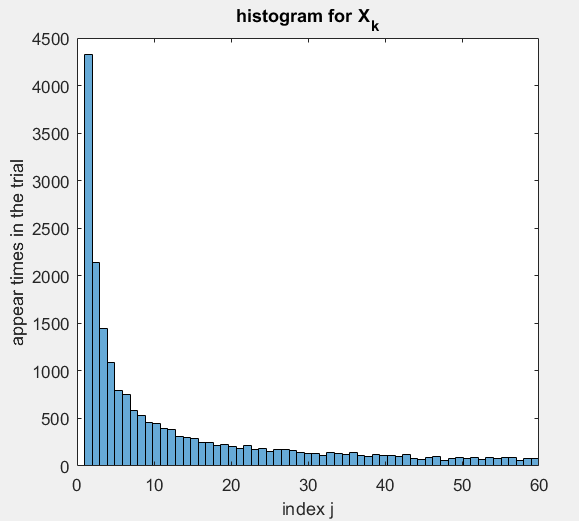
\includegraphics[width = 0.50\textwidth]{../data/solution4.png}  
   \caption{X distribution}
\end{figure}
\noindent \textbf {Analysis}
Using inverse sampling method works well in this situation, because we can see the second bar has half height as the first bar and the third bar has 1/3 height to the first bar which is corresponding to p,p/2,p/3....p/60. Although there seems to be some `noise' when it come to p/45 to p/60(not smmoth enough), given their relatively low probability, such noise can be ignored.\\
\end{multicols}
\subsection{\normalsize{Experiment(b)}}
\noindent The above we have already define a function to generate one X, the requirement in this part is straight forward, if the X is not 60, keep generate X, else stop and record the generate times.\\[10pt]
\underline{\emph{Algorithm}}\\[10pt]
*1.Init times be 0\\
*2.Generate one X\\
*3.X is 60, stop, else times plus one, goto 2\\
*4.Repeat 1,2,3 several times.\\
\noindent \textbf {filename:solution4.m (N\_60 part)}\\
\begin{lstlisting}
%----------------------------------------------------
% N_60 experiment
result_N60 = zeros(1000,1);
for i = 1 : 1000
    N = 0;
    while generateX(p) ~= 60
        N = N +1;
    end
    result_N60(i) = N;
end
figure
histogram(result_N60)
title('histogram for {N_{60}}')
xlabel('the least amount of trials to reach N_{60}')
ylabel('the number of such amount of trials')
Expectation = mean(result_N60);
variance = var(result_N60);
%------------------------------------------------------
\end{lstlisting}
\subsection{\normalsize{Result(b) \&  Analysis}}
\begin{multicols}{2}
\noindent \textbf {Figure \& Data}
\begin{figure}[H]
   \centering
   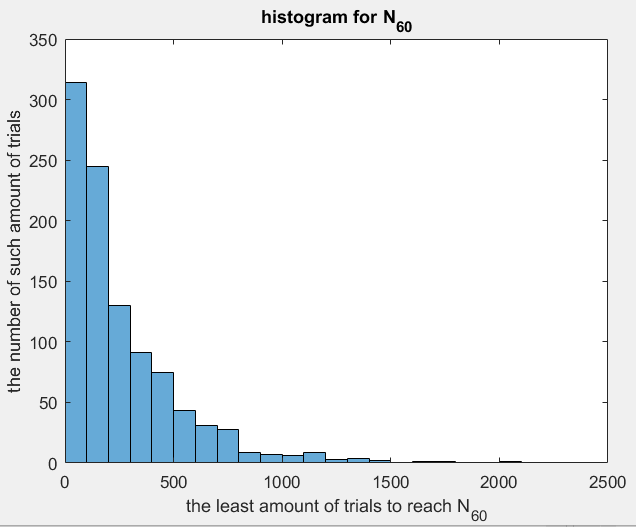
\includegraphics[width = 0.45\textwidth]{../data/solution4_N60.png}  
   \caption{N\_60 Experiment}
\end{figure}
\noindent Expectation = 280.2020\\
\noindent variance = 7.0729e+04.\\
\noindent \textbf {Analysis}\\
This event is actually conform to a geomerty distribution with the probability hitting 60 is p/60, not hitting, $\frac{60-p}{60}$. Therefore, theretical expectation is $\frac{1}{p}$, and the variance $\frac{(1-p)}{p^2}$. In this problem, $p=\frac{p_0}{60}$, and $p_0$ is the normalized one we generated in Experiment(a), which is 0.2137. Therefore, $\mathbb{P}(hit \ 60)= 0.2137/60$.\\
\noindent \textbf {Theoretical expectation:} $1/\mathbb{P}(hit \ 60) = 60/0.2137=280.7674\\$
\noindent \textbf {Experiment expectation: 280.2020.}\\
\noindent \textbf {Theoretical variance}: $(1-\mathbb{P}(hit \ 60))/\mathbb{P}(hit\ 60)^2=7.8563e+04$\\
\noindent \textbf {Experiment variance: 7.0729e+04}\\
\end{multicols}
To sum up, in this experiment, the simulation data conform the theoretical data. Therefore we are doing a experiment which conforms the geometry distribution.\\

\section{Accept-reject method}
\subsection{\normalsize{Problem Description}}
\noindent Use accept-reject method to sample from $p_j$ by sampling from another uniform distribution$q_j$.
\noindent $p_j$ conforms $p_{1 \ to \ 5}=0.06,p_6 = p_9=0.15,p_7=p_10=0.13,p_8=0.14.$\\

\subsection{\normalsize{Experiment:}}
\noindent \textbf {(a):}Understanding the accept-reject method. The rejection sampling method generates sampling values from a target X with arbitrary probability density function f(x) by using a proposal distribution Y with probability density g(x). The idea is that one can generate a sample value from X by instead sampling from Y and accepting the sample from Y with probability ${\displaystyle f(x)/(Mg(x))}$, repeating the draws from Y until a value is accepted. \\
\noindent \textbf {(b):}First, we derive the constant M, M need to be make sure that $Mg(x) > f(x)$ should be true for every x, therefore, we take the max of $(f(x)/g(x))$ to determine the M. Then we using the accept-reject method to derive $f(x)$.\\
\noindent \textbf {(c:)}Overlay the target distribution according to the accepted amount, for example we accept 200 samples in Experiment(b), then the target distribution is [200*0.06,200*0.06,...200*0.14], and compute the efficiency.\\[10pt]
\underline{\emph{Algorithm:}}\\[10pt]
*1. Set distribution q to be {$q_1=0.1,q_2=0.1,\cdots,q_{10}=0.1$}\\
*2. Compute the constant M\\
*3. Generate a rand number i from 1 to 10, generate a number u from std U[0,1]\\
*4. if u< p(i)/Mq(i) , accept and record, else reject.\\
*5. Repeat 3,4 for trail\_budget times.\\
\noindent \textbf {filename: solution5.m}\\
\begin{lstlisting}
function [mean_exp,mean_the,var_exp,var_the,efficiency] = solution5(trial_budget)
%------------------------------------------------------------------------
%usage:[mean_exp,mean_the,var_exp,var_the,efficiency] = solution5(trial_budget)
%trial_budget: the number of times you would like to query for generating
%the sample using accept-reject method
%generate the sample mean and variance using accept-reject method
%generate the theoretical mean and variance
%generate the efficiency of the accept-reject method
%Li Yicheng
%------------------------------------------------------------------------

%accept-reject method
p = [0.06*ones(1,5),0.15,0.13,0.14,0.15,0.13];
%the distribution of p_j
q = ones(1,10)*0.1;
%the distribution to sample from
M = max(p./q);
%derive the coeffience to let all Mq >= p
i=1;
for k = 1 : trial_budget
    y = randi(10);
    u = rand(1);
    if u < p(y)/(M*q(y))
        accept(i) = y;
        i=i+1;
    end
end
%plot part
histogram(accept');
xlabel('index 1 to 10')
ylabel('appear times')
%-------------------------------------------------------------------------
%the target distribution
amount = length(accept);
%to compare the two graph we need to set them have same total sample amount
index = 1;
for i = 1 : 10
    std_distri(index:index + round(amount*p(i))-1)= i*ones(round(amount*p(i)),1);
    %add the 'i's into the sequence, for example in the first loop add
    %(amount * 0.06 ) ones into the sequence from 1 to amount * 0.06;
    index = index + round(amount*p(i));
end
%overlay with the theoretical
hold on
histogram(std_distri);
title('accept-reject sampling')
legend('accept-reject','target')

%the sample mean,variance and the theoretical values
mean_exp = mean(accept);
mean_the = (1:10)*p';
var_exp = var(accept);
var_the = var(std_distri);
%the efficiency
efficiency = amount/trial_budget;
\end{lstlisting}

\subsection{\normalsize{Result \& Analysis}}
\noindent \textbf {query: [m\_exp,m\_the,v\_exp,v\_the,efficiency]= solution5(2000)}\\
\begin{multicols}{2}
\begin{figure}[H]
   \centering
   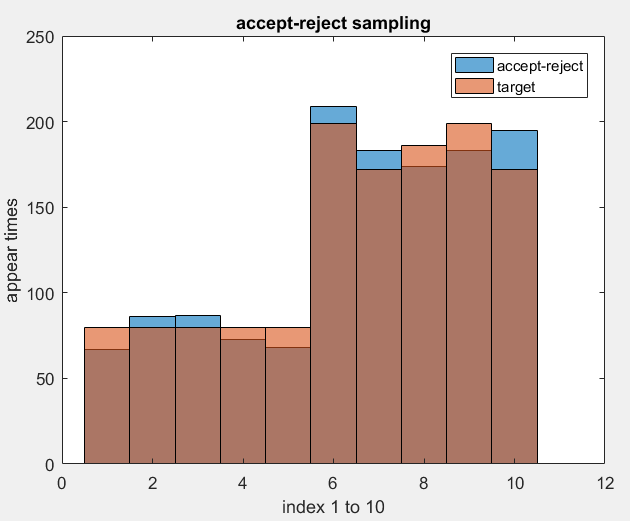
\includegraphics[width =0.5 \textwidth]{../data/solution5.png}  
   \caption{Experiment result \& Target distribution}
\end{figure}
\noindent \textbf {m\_exp=6.3273}\\
\noindent \textbf {m\_the=6.4800}\\
\noindent \textbf {v\_exp=7.7341}\\
\noindent \textbf {v\_the=7.2164}\\
\noindent \textbf {efficiency=0.6630}\\
\noindent \textbf {Theoretical efficience $1/M = 1/(max(p_j/q_j))=1/(0.15/0.1)=1/1.5=0.6666\\$}\\
\end{multicols}
All the data derived from experiment is close to theoretical value. Therefore, accept-reject sampling is also a good method to sample from some ditribution by sampling from another distribution. The only drawback may happen is just the efficiency. Because sometimes we may get a lot of unwanted data. So the choice of  M should be considered if using this method. 
\end{document}